\chapter{The Software}
The complete software consists of the scheduler along with additional supporting
tool and scripts to generate hardware description files and verify the results.
The overall flow of the complete software system including testing and hardware 
description files generation tools is given in the figure.

\begin{figure}[H]
    \centering
    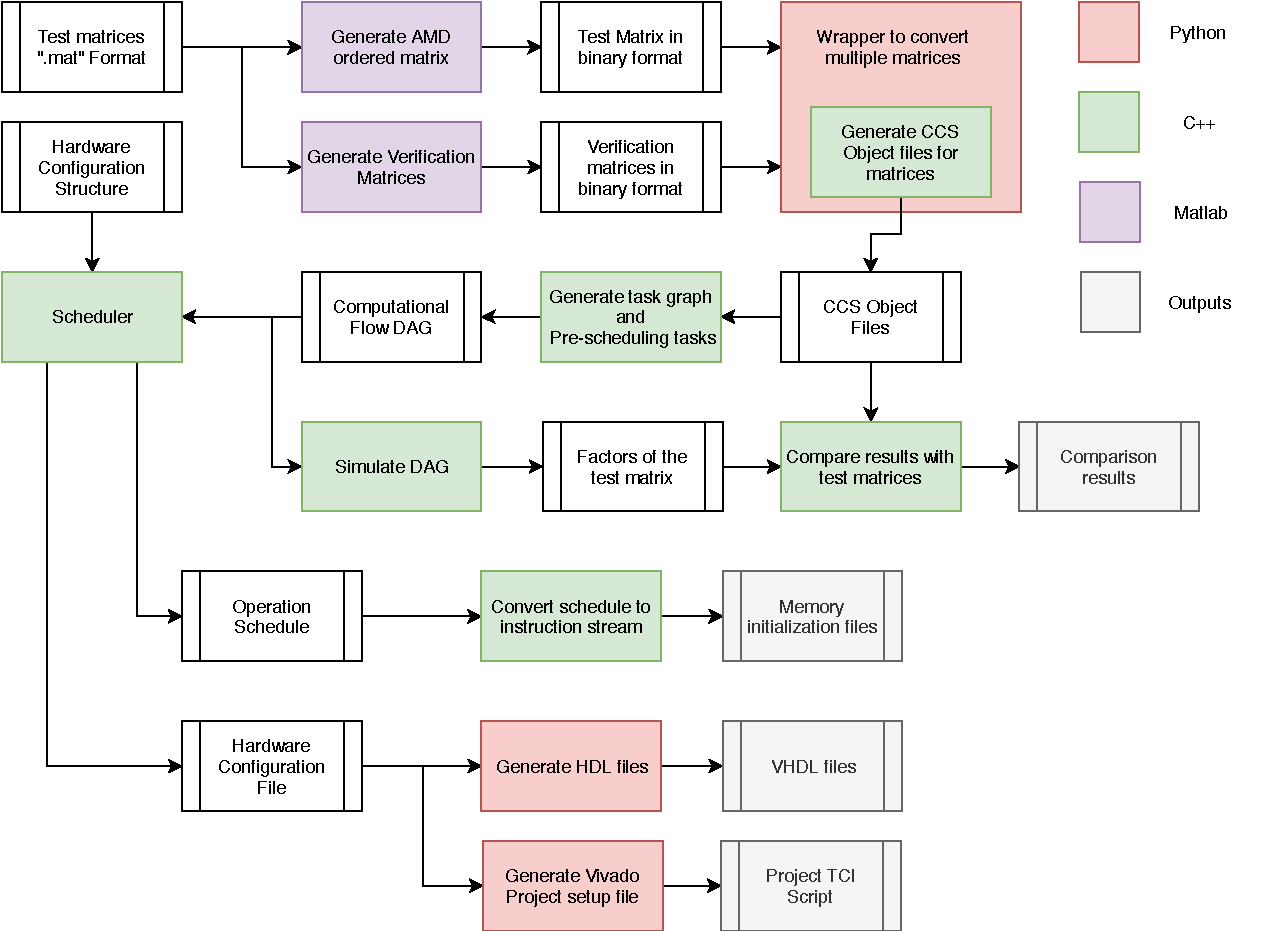
\includegraphics[width = \textwidth]{./Software/softFlow.pdf}
    \caption{Overall flow of the software tool}
    \label{fig:soft:flow}
\end{figure}

\section{Input Processing and Test Generation}
The test matrices are stored in the Matlab structure files. These matrices have to be converted into the 
C++ readable binary format. This is done using a Matlab script which also applies AMD ordering to the 
input matrix. The L and U factors for the input matrix are also generated to be used in the verification stage.
These matrices are stored in the binary file with extension ".sp". This file contains three vectors which represent
matrix in the triplet format. These binary files are then processed by a Python script wrapped around a C++
executable. This converts matrices into the Compressed Column Sparse format and again stores them in binary files 
with extension ".ccs"

\section{HDL Files Generation}
The scheduler program stores the hardware configuration into a ".json" file. This file is read by the 
python script to generate hdl files top entity and multiplexer entities. The scheduler also 
generates memory initialization files for executing the particular matrix. These files are 
used to initialize BRAM data. The second Python script generates project generation 
TCl script. This script includes commands to generate required Xilinx IP packages and 
generating wrappers around them. The script also adds the generated HDL files as well as the simulation 
testbench to the project.

